%!TEX TS-program = xelatex
%!TEX root = ../../maxwell2018thesis.tex

\chapter[Snippet Lengths and Stopping Behaviour]{Snippet Lengths and\\Stopping Behaviour}\label{chap:snippets}
One of the primary components of a retrieval system that searchers interact with the~\glsfirst{acr:serp}. The presentation and design of the~\gls{acr:serp} has over the years been subject to much research. With more complex components now becoming commonplace in contemporary web search engines (such as the \emph{information card}~\citep{navalpakkam2013non_linear_serp, bota2016information_cards} or \emph{social annotations}~\citep{muralidharan2012social_annotations}), much work however still remains on examining how more traditional~\gls{acr:serp} components, such as \emph{result summaries,} are designed and presented to searchers.

\begin{figure}[h]
    \centering
    \vspace{4mm}
    \resizebox{1\hsize}{!}{
    
\includegraphics{figures/ch7-serpintro.pdf}}
    \label{fig:serpintro}
    \vspace{-5mm}
\end{figure}

Result summaries (an example of which is shown above) have been traditionally viewed as the \emph{ten blue links}, each with their corresponding title and source (typically a~\gls{acr:url}) of the document. Included with these two components are the textual \emph{snippets} of \emph{keywords-in-context}, derived from the document itself. These snippets are approximately 130-150 characters (or two lines) in length~\citep{hearst2009_search}. Numerous researchers have explored result summaries in a variety of different ways, such as: examining their length~\citep{paek2004wavelens,cutrell2007eye_tracking,kaisser2008improving}; the use of thumbnails~\citep{woodruff2002summaries,teevan2009visual_snippets}; their attractiveness~\citep{clarke2007caption_features,he2012bridging}; and the generation of \emph{query-biased snippets}~\citep{tombros1998query_biased,rose2007snippet_attributes}. The performance of searchers has broadly been evaluated in a limited fashion (for example, by examining task completion times).

In this chapter, we are interested in examining how the length (and subsequently information content) of result summaries affects~\gls{acr:serp} interactions -- specifically examining their stopping behaviours -- and a searcher's ability to select relevant over non-relevant items. Prior research has demonstrated that longer result summaries tend to lower completion times for informational tasks, where searchers need to find only a single relevant document~\citep{cutrell2007eye_tracking}. Does this finding however hold in an ad-hoc context, where searchers need to find \emph{several} relevant items? Furthermore, how does the length and information associated with longer result summaries affect the searcher's ability to discern the relevant from the non-relevant? We address these questions from the perspective of both:

\begin{itemize}
    \item{a \blueboxbold{user study} examining this phenomenon, as detailed in Section~\ref{chap:snippets:user}; and}
    \item{a \blueboxbold{simulated analysis}, closely examining how varying snippet lengths affects searcher performance and stopping behaviours, discussed in Section~\ref{chap:snippets:simulations}.}
\end{itemize}

The outline for both of these studies follow the general methodology, as discussed in Chapter~\ref{chap:method}. Before discussing the studies and their results, we begin this chapter with an overview of the prior work that has examined the length of result summary snippets.

\section{Background}\label{chap:snippets:background}
As previously discussed, the design and presentation of~\glsplural{acr:serp} has been examined in depth. Researchers have examined various aspects of~\glsplural{acr:serp}, and how the designs of such aspects influence the behaviour of searchers. In this section, we provide a summary of the various aspects that have been examined over time. Specifically, we consider:

\begin{itemize}
    \item{the layout and presentation of~\glsplural{acr:serp};}
    \item{the size of~\glsplural{acr:serp};}
    \item{how snippet text for result summaries is generated; and}
    \item{how much text should be presented within each result summary}.
\end{itemize}

Of the four areas of~\gls{acr:serp} research that we examine in this section, we consider the latter to be the main focus of this work. Each area is summarised below.

\subsection{\gls{acr:serp} Layout and Presentation}
Early works regarding the presentation of result summaries examined different approaches to automatically categorising result summaries for searchers, similar to the categorisation approach employed by early search engines (as shown in Figure~\ref{fig:yahoo} on page~\pageref{fig:yahoo}). ~\cite{chen2000order_to_web} developed an experimental system that automatically categorised result summaries on-the-fly as they were generated. For a query, associated categories were then listed as verticals, with associated document titles provided underneath each category header. Traditional result summaries were then made available when hovering over a document title. Subjects of a user study found the interface easier to use than the traditional \emph{ten blue links} approach -- they were 50\% faster at finding information displayed in categories. This work was then extended by~\cite{dumais2001results_in_context}, where they explored the use of hover text to present additional details about search results based upon user interaction. Searching was also found to be slower with hover text, perhaps due to the fact that searchers were required to consider decision about when to seek additional information explicitly.

Alternatives to the traditional, linear list of result summaries have also been trialled (like grid-based layouts~\citep{resnick2001modeling, kammerer2010interface, chierichetti2011two_dimensional_presentation}). For example,~\cite{kammerer2010interface} examined differences in searcher behaviour when interacting with a standard list interface, compared against a tabular interface (title, snippet and~\gls{acr:url} stacked horizontally in three columns for each result), and a grid-based layout (result summaries placed in three columns). Those using the grid layout spent more time examining result summaries, and demonstrated promise in overcoming issues such as \emph{position bias}~\citep{craswell2008click_models}, as observed by~\cite{joachims2005click_model}.

\cite{marcos2015snippets_web_search} also performed an eye-tracking user study examining the effect of searcher behaviour while interacting with~\glsplural{acr:serp} -- and whether the \emph{richness} of result summaries provided on a~\gls{acr:serp} (i.e. result summaries enriched with metadata from corresponding pages) impacted upon the user's search experience. Enriched summaries were found to help capture a searcher's attention. Including both textual and visual representations of a document when presenting results could have a positive effect on relevance assessment and query reformulation~\citep{joho2006presentation}. Enriched summaries were also examined by~\cite{ali2009interaction_interfaces} in the context of navigational tasks. Striking a good balance between textual and visual cues (i.e. \emph{proximal cues,} as discussed in Section~\ref{sec:stopping_background:models:theoretical:ift}) were shown to better support a searcher's tasks, and search completion time.

\subsection{Generating Snippet Text}
Searchers can be provided with an insight by result summaries as to whether a document is likely to be relevant or not~\cite{he2012bridging}. Consequently, research has been undertaken that examined different kinds of snippets, and how long a snippet should be. Work initially focused upon how these summaries should be generated~\citep{pedersen1991snippet, landauer1993enhancing, tombros1998query_biased, white2003task, leal2015query}. These early works proposed the idea of summarising documents with respect to the query (query-biased summaries), or keywords-in-context -- as opposed to simply extracting the representative or lead sentences from the document~\citep{kupiec1995tds}. Examples of both approaches are illustrated in Figure~\ref{fig:snippet_types}. Indeed,~\cite{tombros1998query_biased} showed that subjects of their study were likely to identify relevant documents more accurately when using query-biased summaries, compared to summaries that were simply generated from the first few sentences of a given document. Query-biased summaries have also been more recently shown to be preferred on mobile devices, too~\citep{spirin2016snippets}.

\begin{figure}[t!]
    \centering
    \resizebox{1\hsize}{!}{
    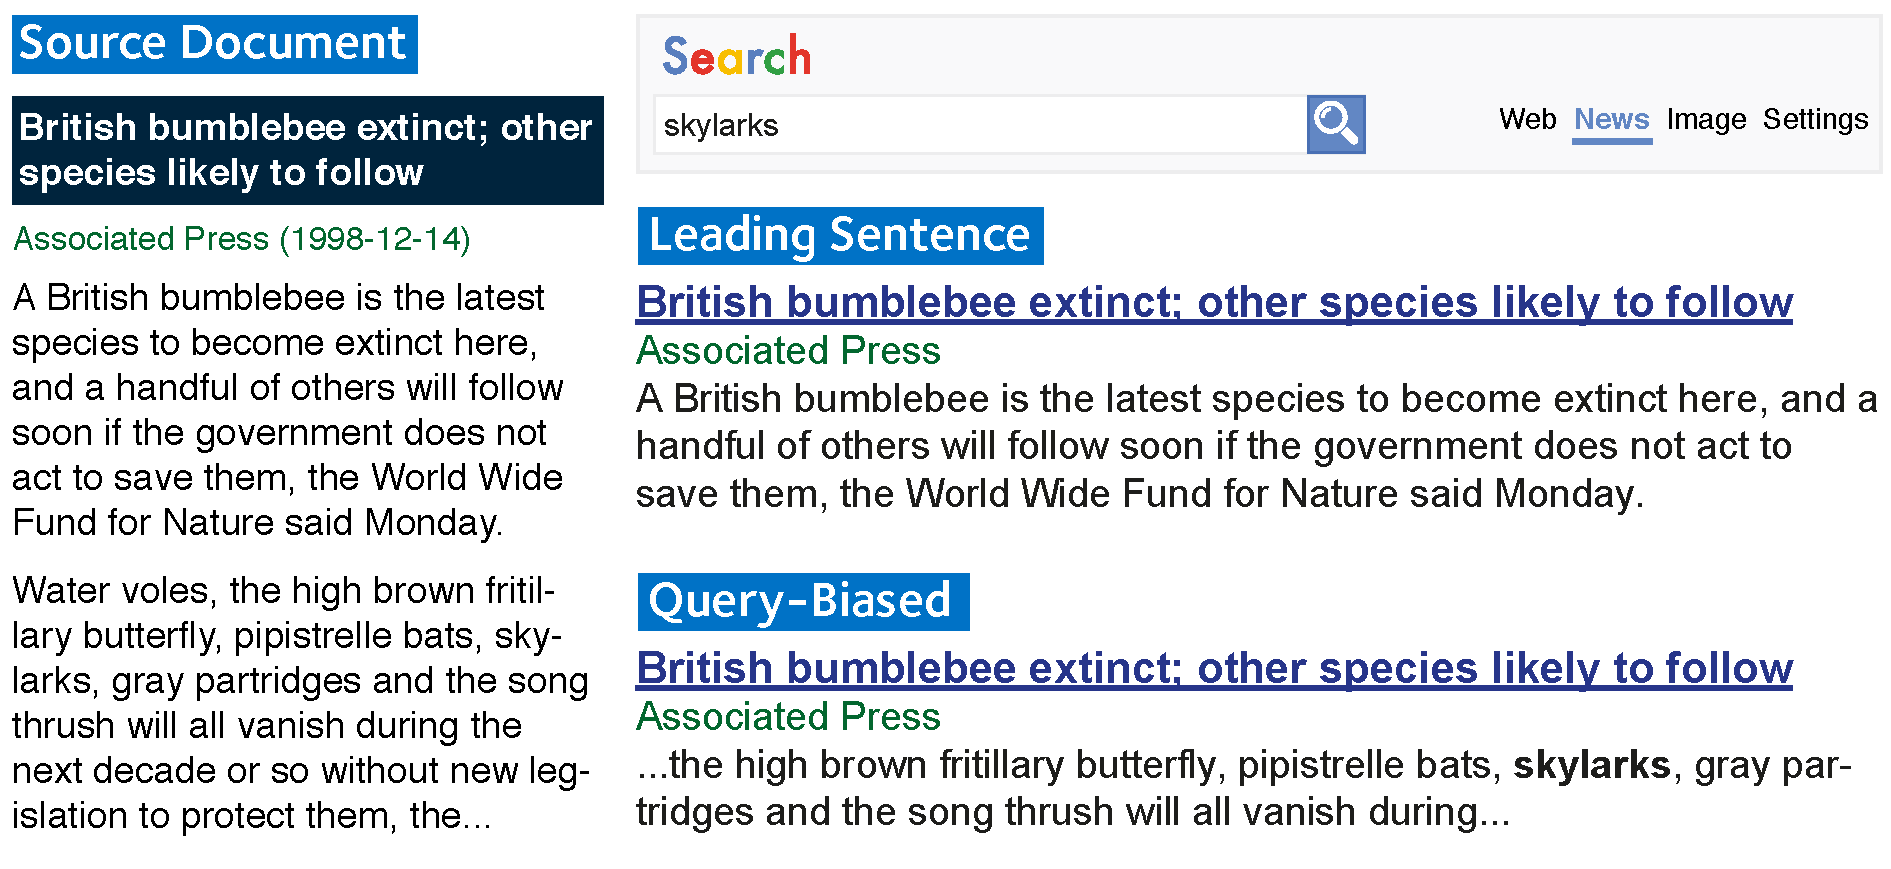
\includegraphics{figures/ch7-snippet_types.pdf}}
    \caption[Leading sentence and query-biased summary examples]{A visual example of two different types of summary, along with a portion of an example document from the~\gls{acr:trec} AQUAINT collection. Given the query \texttt{skylarks}, the \searchlogo~result summaries for both leading sentence and query-biased summaries are shown. Note the highlighting of the term \textbf{skylarks} in the query-biased summary.}
    \label{fig:snippet_types}
\end{figure}

When constructing snippets using query-biased summaries,~\cite{rose2007snippet_attributes} found that a user's perceptions of the result's quality were influences by the snippets. If snippets contained truncated sentences or many fragmented sentences (denoted as \emph{text choppiness}), searchers perceived the quality of the results more negatively, regardless of length.~\cite{kanungo2009snippet_readability} found that poor readability also impacted upon how the resultant snippets were perceived. They maintain that readability is a crucial presentation attribute that needs to be considered when generating a query-biased summary.~\cite{clarke2007caption_features} analysed thousands of pairs of snippets where result \emph{A} appeared before result \emph{B}, but result \emph{B} received more clicks than result \emph{A.} As an example, they found results with snippets which were very short (or missing entirely) had fewer query terms, were not as readable, and attracted fewer clicks. This led to the formulation of several heuristics relating to document surrogate features, designed to emphasise the relationship between the associated page and generated snippet. Heuristics included:

\begin{itemize}
    \item{ensuring that all query terms appeared in the generated snippet (where possible);}
    \item{withholding the repeating of query terms in the snippet if they were present in the page's title; and}
    \item{displaying shortened, easily readable~\glsplural{acr:url}.}
\end{itemize}

Recent work has examined the generation of snippets from more complex angles -- from manipulating underlying indexes~\citep{turpin2007fast_snippets, bast2014snippet_generation}, to language modelling~\citep{li2010snippet_extraction, he2012bridging}, as well as using a searcher's recorded history to improve the snippet generation process~\citep{ageev2013summaries, savenkov2011search}. Previous generation approaches also may not consider what parts of a document searchers actually find useful.~\cite{ageev2013summaries} incorporated into a new model post-click searcher behaviour data, such as mouse cursor movements and scrolling over documents, producing \emph{behaviour-based snippets.} Results showed a marked improvement over a strong text-based snippet generation baseline. Temporal aspects have also been considered --~\cite{svore2012temporal_snippets} conducted a user study that showed searchers preferred snippet text with \emph{trending} content in snippets when searching for trending queries, but not so for general queries.

\subsection{Results per Page}
Today, a multitude of devices are capable of accessing the~\gls{acr:www} -- along with a wide range of different screen resolutions and aspect ratios. The question of how many result summaries should be displayed per page therefore becomes hugely important, yet increasingly difficult to answer. Examining behavioural effects of mobile devices when interacting with~\glsplural{acr:serp} has attracted much research as of late (e.g.~\cite{kim2012small_vs_large, kim2014eye_tracking, kim2016pagination_versus_scrolling}), and with each device capable of displaying a different number of results \emph{above-the-fold}\footnote{Refer to Section~\ref{chap:csm:method:simulation:grounding:serp} for a detailed explanation on displaying results \emph{above-the-fold.}}, recent research has shown that the number of results shown per page can influence the behaviour of searchers~\citep{joachims2005click_model, kim2014eye_tracking}. Understanding this behaviour can help guide and inform those charged with designing contemporary retrieval system user interfaces.

In a Google industry report,~\cite{linden2006} however stated that searchers desired more then 10 results per page, despite the fact that increasing the number of results displayed yielded a 20\% drop in traffic. It was hypothesised that this was due to the extra time required to dispatch the longer~\glsplural{acr:serp}. This drop however could have been attributed due to other reasons.~\cite{oulasvirta2009serp_size} discussed the \emph{paradox of choice}~\citep{schwartz2005paradox_of_choice} in the context of search, where more options (results) -- particularly if highly relevant -- will lead to poorer decisions, degrading searcher satisfaction. In terms of searcher satisfaction, it can be argued that modern search engines can therefore be a victim of their own success, leaving searchers with \emph{choice overload.}~\cite{oulasvirta2009serp_size} found that presenting searchers with a six-item result list was associated with higher degrees of searcher satisfaction, confidence with choices and perceived carefulness than a list of 24 items.

\cite{kelly2015serp_size} broadly agreed with the findings of~\cite{oulasvirta2009serp_size}. Here, the authors conducted a between-subjects study with three conditions, where subjects were assigned to one of three interfaces -- a baseline interface, showing 10 results per page (the traditional \emph{ten blue links}), and two interfaces displaying 3 and 6 results per page respectively. Their findings showed that individuals using the 3 and 6 results page page interfaces spent significantly longer examining top ranked results, and were more likely to click on higher ranked documents than those using the 10 results per page interface. Findings from this study also suggested that subjects using the interfaces showing fewer results per page found it comparatively easier to find relevant content than those using the 10 results per page interface. However, no significant difference was found between the number of relevant items found across the interfaces. As we have discussed previously throughout this thesis, 10 results per page is still considered the \emph{de-facto} standard~\citep{hearst2009_search}.

\subsection{Snippet Lengths: Longer or Shorter?}
Snippet lengths have been examined in a variety of ways. A user study by~\cite{paek2004wavelens} compared a searcher's preference and usability against three different interfaces for displaying result summaries. With question answering tasks, the interfaces:

\begin{itemize}
    \item{displayed a \emph{normal}~\gls{acr:serp}, consisting of a two line snippet for reach result summary, complete with a clickable hyperlink to the corresponding document;}
    \item{an \emph{instant} interface, where an expanded snippet was displayed upon clicking it; and}
    \item{a \emph{dynamic} interface, where hovering the cursor would trigger the expanded snippet.}
\end{itemize}

The instant view was shown to allow searchers to complete the given tasks in less time than the normal baseline, with half of participants preferring this approach.

Seminal work by~\cite{cutrell2007eye_tracking} explored the effect of different snippet lengths, exploring \emph{short} (1 line), \emph{medium} (2-3 lines, the expected standard) and \emph{long} (6-7 lines) snippets. They found that longer snippets significantly improved performance for \emph{informational tasks} (e.g. \texttt{find the address for Glasgow International Airport}). Searchers performed better for informational queries as snippet length increased. This work was followed up by~\cite{kaisser2008improving}. They conducted two experiments that estimated the preferred snippet length according to answer type (e.g. finding a person, time, or place), and comparing the results of the preferred snippet lengths to searchers' preferences to see if this could be predicted. This preferred snippet length was shown to depend upon the type of answer expected, with greater searcher satisfaction shown for the snippet length predicted by their technique. Findings also indicated that longer snippets could be more useful if the snippet was considered relevant to the query issued.

More contemporary work has begun to examine what snippet sizes are appropriate for mobile devices, with the multitude of screen resolutions available. Given smaller screen sizes when compared to desktop or laptop computers, this is particular important -- snippet text considered acceptable on a computer screen may involve considerable scrolling/swiping on a smaller screen.~\cite{kim2017mobile_search_snippets} found that subjects using longer snippets on mobile devices exhibited longer search times and similar search accuracy under informational tasks.\footnote{The tasks considered by~\cite{kim2017mobile_search_snippets} were similar to those defined by~\cite{cutrell2007eye_tracking}, where a single relevant document was sought.} Longer reading times and frequent scrolling/swiping (with more viewport movement) were exhibited. Longer snippets did not therefore appear to be very useful on a small screen -- an \emph{instant} or \emph{dynamic} approach (as per~\cite{paek2004wavelens}) may have practical application for mobile search, too.

\section{Varying Snippet Lengths}\label{chap:snippets:user}
As can be seen from the background to this chapter, the presentation of result summaries has been demonstrated to have a strong effect on the ability of a searcher to judge relevancy~\citep{he2012bridging}. Relevant documents may be overlooked due to uninformative or unattractive summaries -- but conversely, non-relevant documents may be examined due to a misleading summary, too. Longer summaries also however increase the cost of examination, so there is likely a tradeoff between informativeness/accuracy and length/cost. The current, widely accepted standard for result summaries are \emph{two query-biased snippets/lines}~\citep{hearst2009_search}. As discussed earlier in Chapter~\ref{chap:snippets} however, does this hold under an ad-hoc context? Under this context, do searchers, when presented with longer summaries, obtain a better ability to discern the relevant from the non-relevant?

To address these questions, we in this section discuss a user study that served as an investigation into the effects of search behaviour -- particularly stopping behaviours -- and search performance when we varied result summary snippet lengths, and by doing so, the information content presented within the summaries. Following the general methodology of our two user studies outlined in Section~\ref{sec:method:user_study}, the user study reported is crowdsourced ($n=53$) and within-subjects. Under ad-hoc topic retrieval, participants used four different search interfaces, each with a different size of result summary. Findings from this study allowed us to address two main research questions, which we enumerate below.

\begin{itemize}
    \item{\blueboxbold{RQ1} How does the value of information gain, represented as snippet length, affect searcher behaviour, performance and user experience?}
    \item{\blueboxbold{RQ2} Does information gain -- again represented as snippet length -- affect the decision making ability and ability to identify relevant documents of searchers?}
\end{itemize}

We hypothesised that longer and more informative result summaries would enable participants to make better quality decisions, being more informed with a greater volume of text. In the remainder of this section, we:

\begin{itemize}
    \item{discuss the methodology of the study, discussing the study-specific aspects of the experimental design to complement the general methodology outlined in Section~\ref{sec:method:user_study};}
    \item{provide results and analysis from the study, providing insight into the two study-specific research questions outlined above;}
    \item{discuss the implications of the study.}
\end{itemize}

We then take the interaction data from this study forward to Section~\ref{chap:snippets:simulations}, using it as a means of grounding a series of simulations to examine in greater depth how snippet length affects searcher stopping behaviours.

\subsection{Methodology}
In this section, we outline the methodology employed for this user study. This section provides study-specific, supplementary details to the general user study methodology that was outlined in Section~\ref{sec:method:user_study}. This general user study methodology is employed here, and in the subsequent user study discussed in Chapter~\ref{chap:diversity}. For each subsection discussed below, we refer back to the relevant section in the general methodology to assist in understanding how each of the different components fit together.

Below, we discuss the different search interfaces that we trialled, along with how we generated result summary snippets of varying length. We then provide a brief discussion of the $53$ subjects who took part in the user study, explain the search task, and discuss the post-task surveys that subjects completed.

\subsubsection{Search System and Interfaces}
In conjunction with the common retrieval system, corpus and topics discussed in Section~\ref{sec:csm:methodology:collection}, we trialled four different search interfaces as part of the within-subjects study design. The four interfaces presented snippets, as part of result summaries, of varying lengths. This allowed us to explore the influence of snippet length and snippet informativeness on search behaviours, performance and user experience.

\begin{wrapfigure}[5]{r}{0.45\textwidth}
    \begin{center}
    \vspace*{-10mm}
    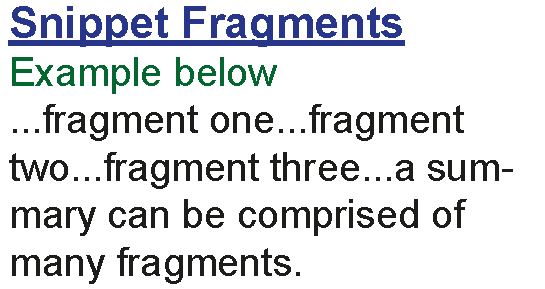
\includegraphics[width=1\textwidth]{figures/ch7-fragments.pdf}
    \end{center}
    \vspace*{-4mm}
    \label{fig:fragments}
\end{wrapfigure}

To decide the length and informativeness of the result summaries, we performed a preliminary analysis to determine the average length (in words) and informativeness (as calculated by the~\glsfirst{glos:kl}~\citep{kullback1951information} \todo{distance} to measure \emph{information gain}, or \emph{relative entropy}) of result summaries with the title, and a varying number of \emph{snippet fragments}\footnote{Figure~\ref{fig:serp_example} on page~\pageref{fig:serp_example} illustrates snippet fragments in the wider context of a~\gls{acr:serp}.} (from $0$ to $10$). The closer the entropy value is towards zero, the more information that is gained. Figure~\ref{fig:ig_plots} plots the number of words, the information gain, and the information gain attained per word.\footnote{These values were obtained by submitting over $300$ queries from a previous user study, conducted by~\cite{azzopardi2013query_cost}. These were conducted on similar topics, the same retrieval system and corpus used as the those used for this study.} It is clear from the plots shown in Figure~\ref{fig:ig_plots} that a higher level of information gain was present in longer snippets. However, as the length increased with each snippet fragment added, the informativeness per word also decreased. Consequently, we selected the four different interface conditions in the region where informativeness has the highest change, i.e. from zero to four. The conditions selected for this study were therefore:

\begin{figure}[t!]
    \centering
    \resizebox{1\hsize}{!}{
    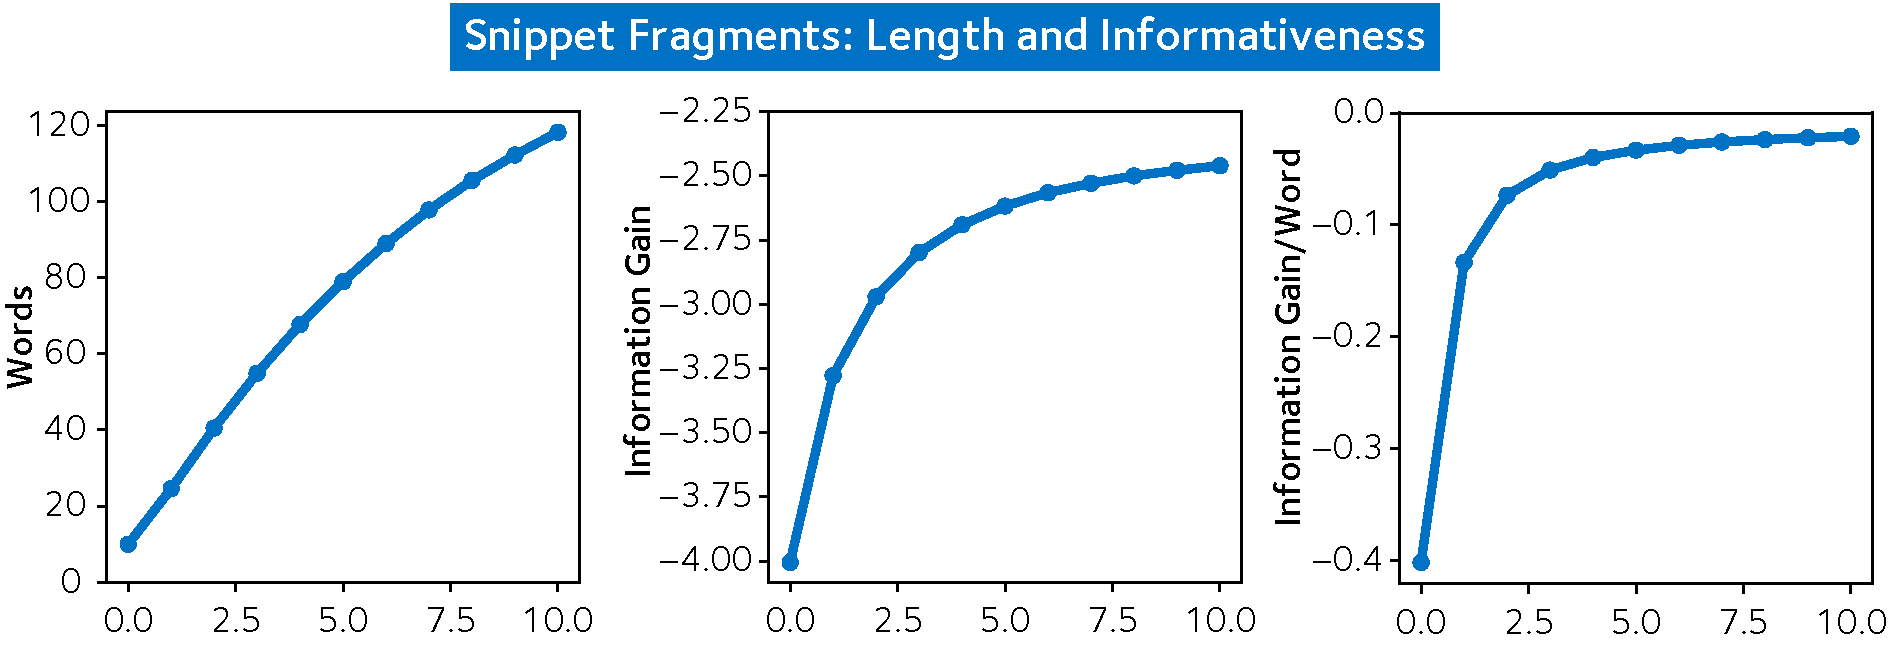
\includegraphics{figures/ch7-ig_plots.pdf}}
    \caption[Information gain plots]{Plots showing the length (in words), informativeness (in information gain, or \emph{IG}), and the information gain \emph{(IG)} per word for the title, plus 0 to 10 snippet fragments. The closer the value is to zero, the more information that is gained.}
    \label{fig:ig_plots}
\end{figure}

\begin{itemize}
    \item{\blueboxbold{T0}, where only the title for each result summary were presented;}
    \item{\blueboxbold{T1}, where for each result summary, a title and one query-biased snippet fragment were presented;}
    \item{\blueboxbold{T2}, where a title and two query-biased snippet fragments were presented; and}
    \item{\blueboxbold{T4}, where a title and four query-biased snippet fragments were presented.}
\end{itemize}

For these interfaces, our independent variable was snippet informativeness, controlled by the length of the result summary snippets. \todo{Figure~\ref{}} provides an example of the different result summaries in each condition, using the same document.

\begin{figure}[t!]
    \centering
    \resizebox{1\hsize}{!}{
    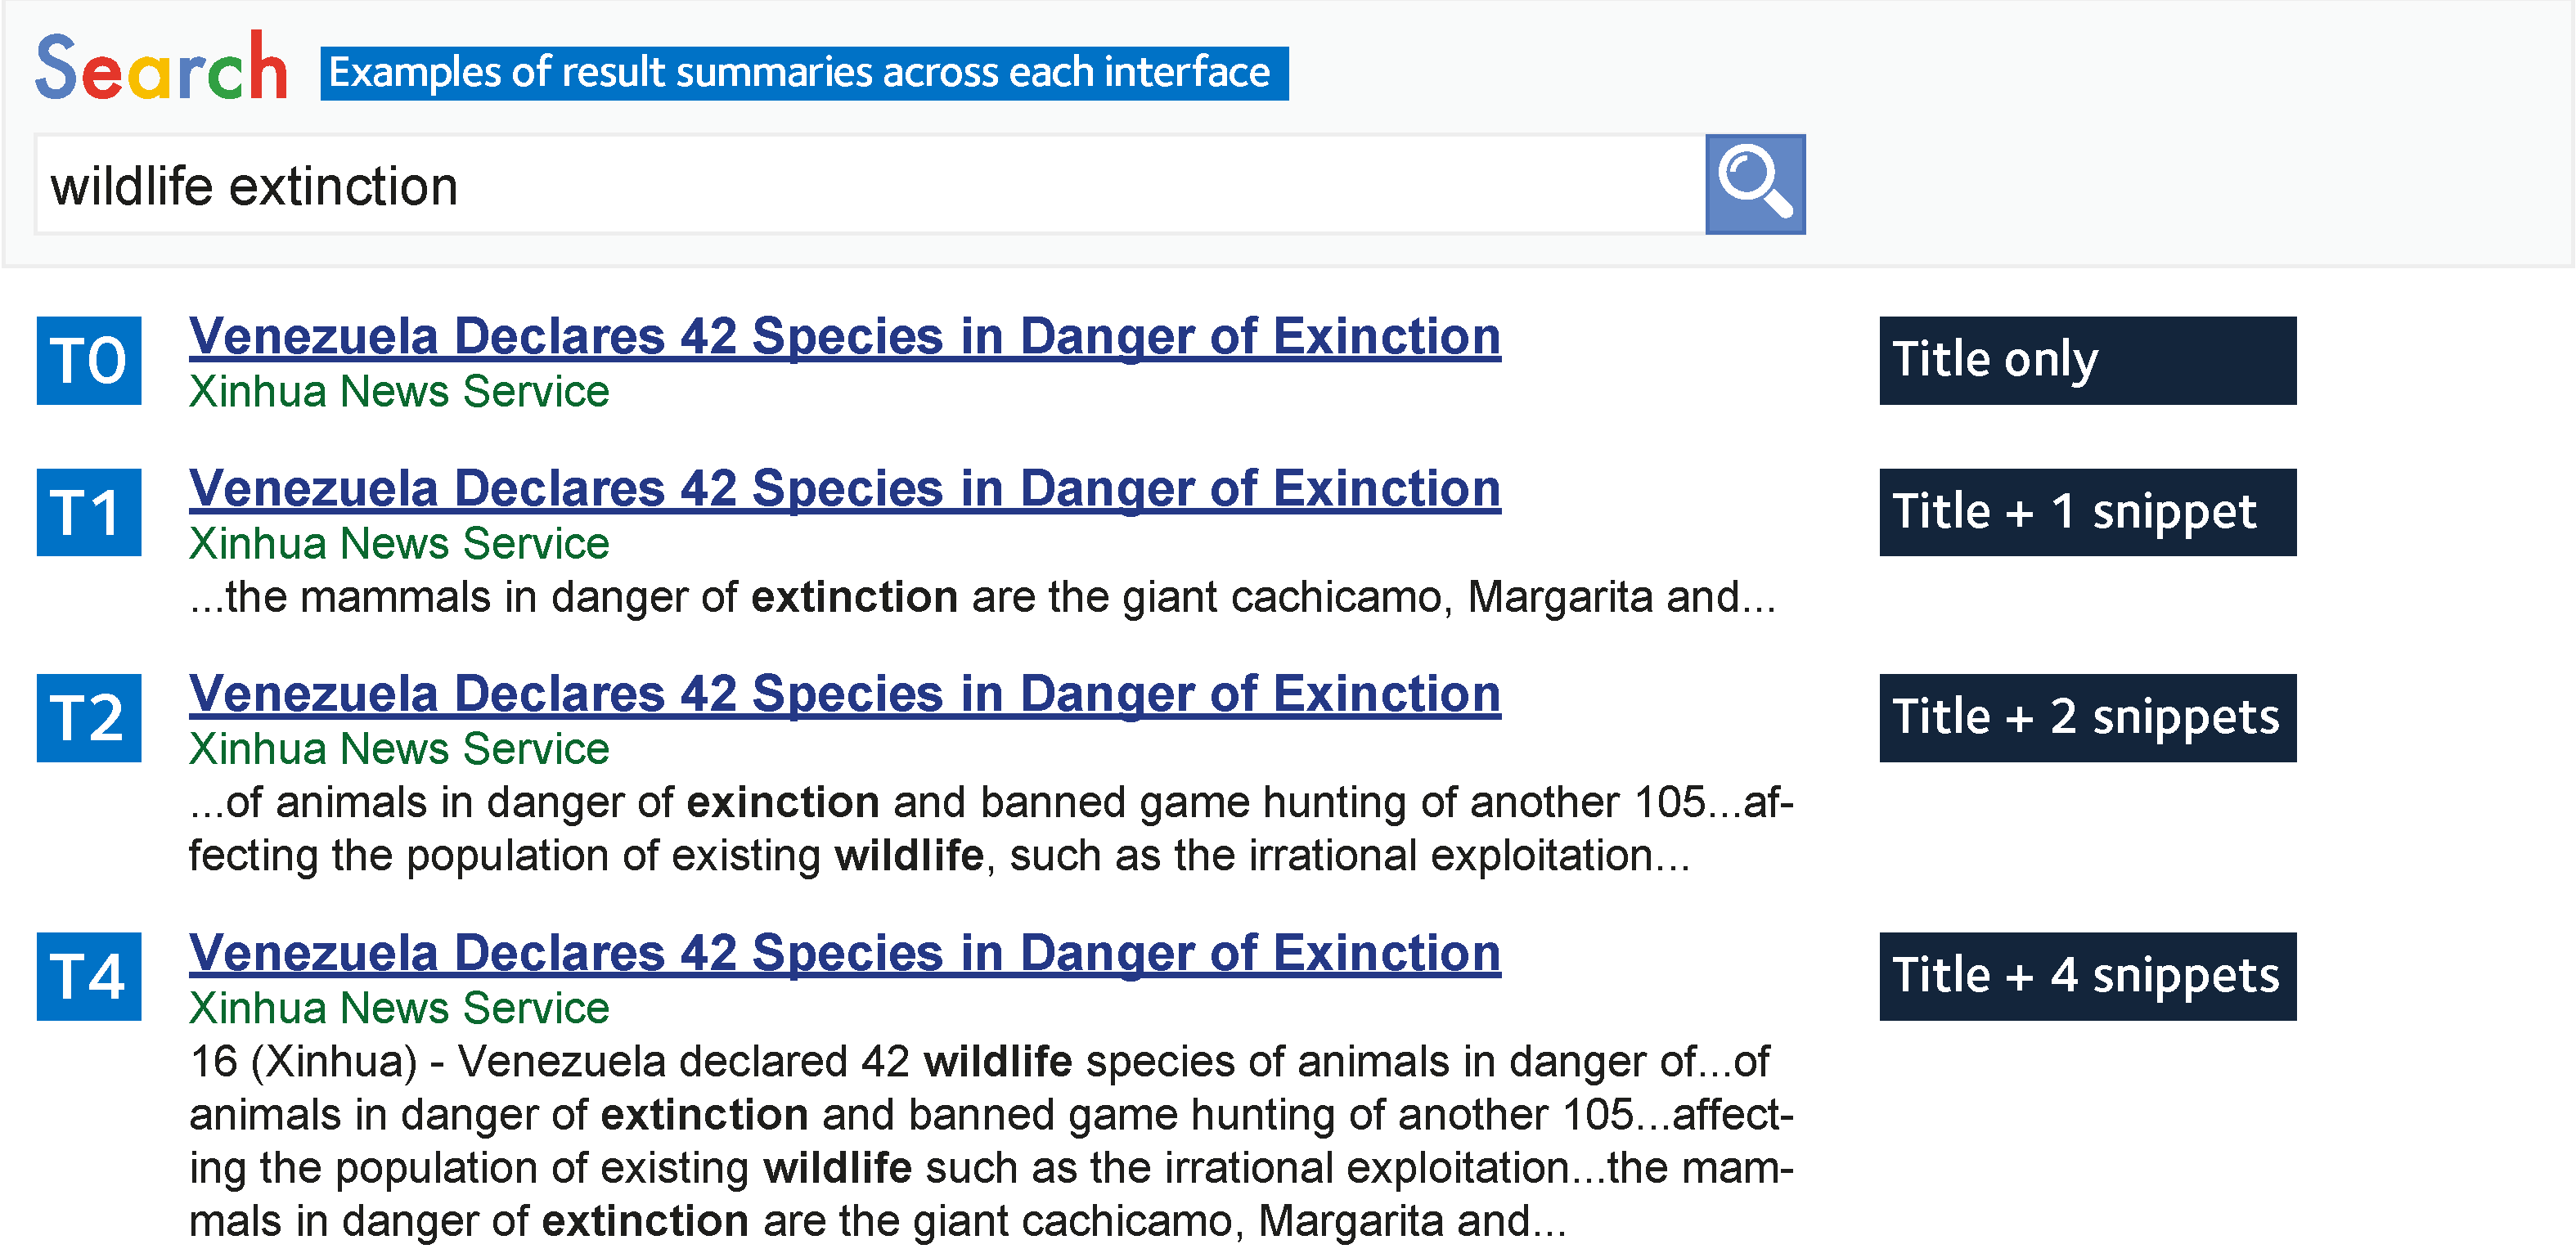
\includegraphics{figures/ch7-interface_snippets.pdf}}
    \caption[Examples of result summaries from the four interfaces]{Examples of the result summaries generated by each of the four interfaces, \blueboxbold{T0}, \blueboxbold{T1}, \blueboxbold{T2} and \blueboxbold{T4} used in this study. The same document is used. Demonstrated by \searchlogo, each of the result summaries consists of a title (in blue, underlined), none, one, or more snippet fragments (in black, with fragments separated by ellipses), and a newswire source (in green).}
    \label{fig:interface_snippets}
\end{figure}

From here, we carefully selected the order in which subjects were presented with each interface. For each of the four main topics discussed in Section~\ref{sec:csm:methodology:collection}, one of the four interfaces from \blueboxbold{T0}, \blueboxbold{T1}, \blueboxbold{T2} and \blueboxbold{T4} were assigned using a Latin-square rotation. For the practice topic, we used \blueboxbold{T2} -- the interface that represented the \emph{de facto} standard for presenting result summaries~\citep{hearst2009_search}.

\subsubsection{Snippet Generation}
WHAT IS A FRAGMENT? Look at Figure~\ref{fig:serp_example} on page~\pageref{fig:serp_example} for an example of this.

\subsubsection{Subjects and Search Task}

\subsubsection{Post-Task Surveys}


\subsection{Results and Analysis}

\subsubsection{Interactions}

\subsubsection{Performance}

\subsubsection{Time-Based Measures}

\subsubsection{User Experience}

\subsection{Discussion}

\section{Simulated Analysis}\label{chap:snippets:simulations}

\subsection{Methodology}

\subsubsection{Interaction Costs and Probabilities}

\subsection{Results}

\subsubsection{Performance}

\subsubsection{Comparisons}

\subsubsection{Discussion}

\section{Chapter Summary}